\documentclass[12pt,aspectratio=43]{beamer}

% 自訂字體的封包
\usepackage{fontspec}

% 導入圖形與表格的封包
\usepackage{graphicx}
\graphicspath{{./20251203_Meeting}}

\usepackage{booktabs}

% 排列多個子圖形的封包
\usepackage{subfigure} 

 % 提供進階數學環境與公式排版
\usepackage{mathtools, amsmath, amsfonts, amsthm, latexsym} 

%% 設定中文字體
\usepackage{xeCJK}
\setCJKmainfont[AutoFakeBold=3.5 , AutoFakeSlant=0.2]{標楷體}
\setmainfont{Times New Roman}
\XeTeXlinebreaklocale "zh"
\XeTeXlinebreakskip = 0pt plus 1pt

% 自訂字體顏色的封包
\usepackage{color} 

% 圖表自動編號的封包
\usepackage{caption} 

% 允許表格的一格能多列呈現的封包
\usepackage{multirow} 

% 可指定表格排版的封包
\usepackage{array}

% 翻轉表格的封包
\usepackage{lscape} 

% 序列標號
\usepackage{enumerate} 

%% 設定自動編號
\setbeamertemplate{caption}[numbered]

%% 自訂顏色
\definecolor{Myblue}{RGB}{57,108,144}
\definecolor{Default_Blue}{RGB}{52,51,171}

% (動畫)字會若隱若現的顯示
\beamersetuncovermixins{\opaqueness<1->{45}}{\opaqueness<1->{95}} 

% 設定中文的標籤
\renewcommand{\figurename}{圖} 
\renewcommand{\tablename}{表} 

% 排版形式 
\mode<presentation>{
\usetheme{Berlin}
% enumerate 及 item 的形狀
\setbeamertemplate{itemize items}[triangle]
% 調整外框形式的字體大小
\setbeamerfont{headline}{size=\scriptsize}
\setbeamerfont{footline}{size=\scriptsize}
% 取消右下方的跳轉工具列
\setbeamertemplate{navigation symbols}{} 
% 自定義2：清除外框下緣但僅出頁碼
\setbeamertemplate{footline}[page number] 
% 顏色主題
\usecolortheme{dove}
% 設定頁面邊界
\setbeamersize{text margin left=0.6cm, text margin right=0.6cm}
\special{papersize=\the\paperwidth,\the\paperheight}
\providecommand{\tabularnewline}{\\}
}

\title{Meeting 1203}
\author{黃丞暘}
\institute{國立東華大學應數統計所}
\date{December 03, 2025}

\begin{document}

% 封面
\begin{frame}
  \titlepage
\end{frame}

% 目錄
\begin{frame}{\textbf{Index}}
  \tableofcontents
\end{frame}

% 研究動機 
\section{11.26 Discussion}

\begin{frame}{\textbf{11.26 Discussion}}
\linespread{1.5}
  Semiconductor Manufacturing Process
  \begin{itemize}
    \item 抽掉outlier讓PCA更散更清楚
  \end{itemize}
  \begin{itemize}
    \item (Yi, Xi)~iid F(•)
  \end{itemize}
\end{frame}

% 研究方法
\section{11.26 Todo}

\begin{frame}{\textbf{11.26 Todo}}
\linespread{1.5}
  \begin{itemize}[]
    \item 繼續分成幾群再套模型比較最合適的
  \end{itemize}
  \begin{itemize}[]
    \item 對outlier做質性的統計方法
  \end{itemize}
  \begin{itemize}[]
    \item 在降維分群之前做SMOTE看看效果
  \end{itemize}
\end{frame}

% 結果
\section{Resulut - What I do this time}

\begin{frame}{\textbf{Results I}　{PCA + KMeans, 2 clusters}}
\linespread{0.9}

\begin{center}
\begin{minipage}{0.3\linewidth}
	\centering
	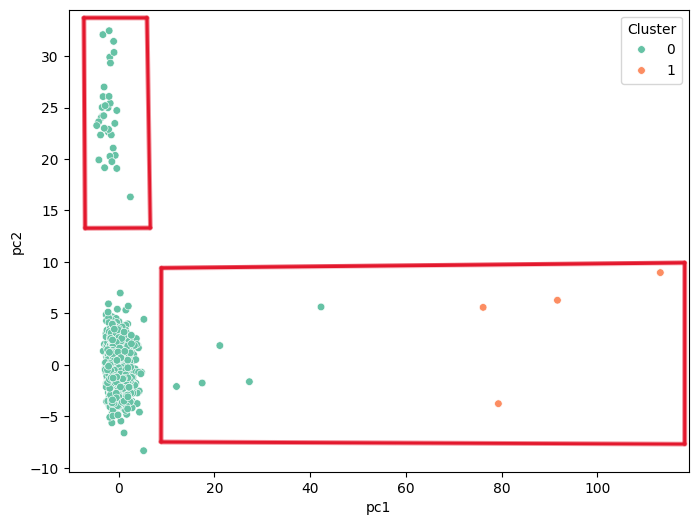
\includegraphics[width=\linewidth]{PCA0r3.png}
\end{minipage}
\hspace{0.3em}
\begin{minipage}{0.55\linewidth}
	\centering
	
\includegraphics[width=\linewidth]{PCA1.png}
\end{minipage}
\end{center}

\small{$$
\begin{array}{c|cc}
\text{cluster} & 0 & 1 \\
\hline
y=0 & 660 & 770 \\
y=1 & 58  & 37 \\
\end{array}
$$}

\end{frame}

\begin{frame}{\textbf{Results I}　{5-folds cv - mean}}
\linespread{0.9}

{\small
Summary
$$
\begin{array}{l|ccc}
\text{model} 
& \text{ACC} & \text{FAR} & \text{ROCAU}\\
\hline
\text{LR}  & 0.8551 & 0.0977 & 0.5476\\
\text{SVM} & 0.9292 & 0.0048 & 0.4976\\
\text{DT}  & 0.8264 & 0.1292 & 0.5366\\
\text{RF}  & 0.9317 & 0.0027 & 0.5036\\
\text{XGB} & 0.9247 & 0.0130 & 0.5176\\
\end{array}
$$
}

{\small
$$
\begin{array}{l|ccc|ccc}
\text{model} 
& \text{$C_0$ACC} & \text{$C_0$FAR} & \text{$C_0$ROCAU} 
& \text{$C_1$ACC} & \text{$C_1$FAR} & \text{$C_1$ROCAU}\\
\hline
\text{LR}  & 0.8315 & 0.1136 & 0.5470 & 0.9021 & 0.0636 & 0.5593\\
\text{SVM} & 0.9178 & 0.0015 & 0.4992 & 0.9542 & 0.0000 & 0.5000\\
\text{DT}  & 0.7967 & 0.1561 & 0.5515 & 0.8773 & 0.0896 & 0.5481\\
\text{RF}  & 0.9178 & 0.0015 & 0.4992 & 0.9554 & 0.0000 & 0.5143\\
\text{XGB} & 0.9081 & 0.0182 & 0.5258 & 0.9554 & 0.0000 & 0.5143\\
\end{array}
$$
}
\end{frame}

\begin{frame}{\textbf{Results II}　{PCA + KMeans, 3 clusters}}
\linespread{0.9}

\begin{center}
\begin{minipage}{0.3\linewidth}
	\centering
	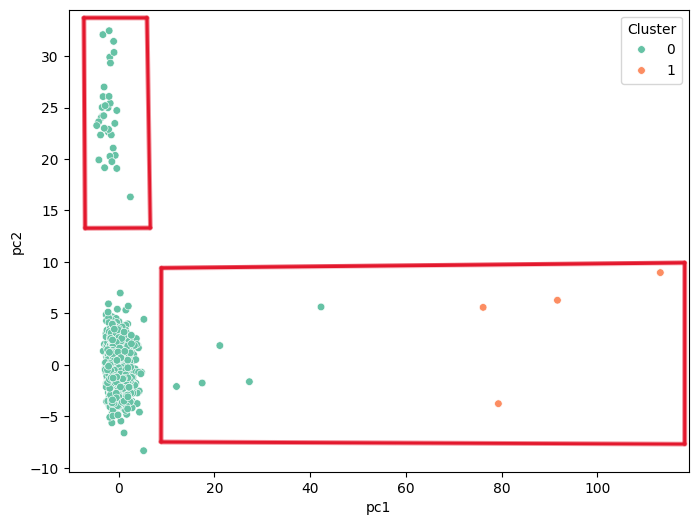
\includegraphics[width=\linewidth]{PCA0r3.png}
\end{minipage}
\hspace{0.3em}
\begin{minipage}{0.55\linewidth}
	\centering
	
\includegraphics[width=\linewidth]{PCA2.png}
\end{minipage}
\end{center}

\small{$$
\begin{array}{c|ccc}
\text{cluster} & 0 & 1 & 2\\
\hline
y=0 & 592 & 327 & 511\\
y=1 & 49 & 19 & 27 \\
\end{array}
$$}

\end{frame}

\begin{frame}{\textbf{Results II}　{5-folds cv - mean}}
\linespread{0.9}

{\small
$$
\begin{array}{l|ccc|ccc}
\text{model} 
& \text{$C_0$ACC} & \text{$C_0$FAR} & \text{$C_0$ROCAU} 
& \text{$C_1$ACC} & \text{$C_1$FAR} & \text{$C_1$ROCAU}\\
\hline
\text{LR}  & 0.8346 & 0.1082 & 0.5170 & 0.8872 & 0.0673 & 0.5247\\
\text{SVM} & 0.9236 & 0.0000 & 0.5000 & 0.9422 & 0.0031 & 0.4985\\
\text{DT}  & 0.8081 & 0.1436 & 0.5415 & 0.8555 & 0.1042 & 0.5229\\
\text{RF}  & 0.9235 & 0.0017 & 0.5092 & 0.9451 & 0.0000 & 0.5000\\
\text{XGB} & 0.9142 & 0.0135 & 0.5132 & 0.9335 & 0.0122 & 0.4939\\
\end{array}
$$
}

{\small
$$
\begin{array}{l|ccc}
\text{model} 
& \text{$C_2$ACC} & \text{$C_2$FAR} & \text{$C_2$ROCAU}\\
\hline
\text{LR}  & 0.9183 & 0.0470 & 0.6032\\
\text{SVM} & 0.9498 & 0.0000 & 0.5000\\
\text{DT}  & 0.8755 & 0.0900 & 0.5683\\
\text{RF}  & 0.9498 & 0.0000 & 0.5000\\
\text{XGB} & 0.9405 & 0.0137 & 0.5298\\
\end{array}
$$
}


\end{frame}

\begin{frame}{\textbf{Results III}　{PCA + KMeans, 4 clusters}}
\linespread{0.9}

\begin{center}
\begin{minipage}{0.3\linewidth}
	\centering
	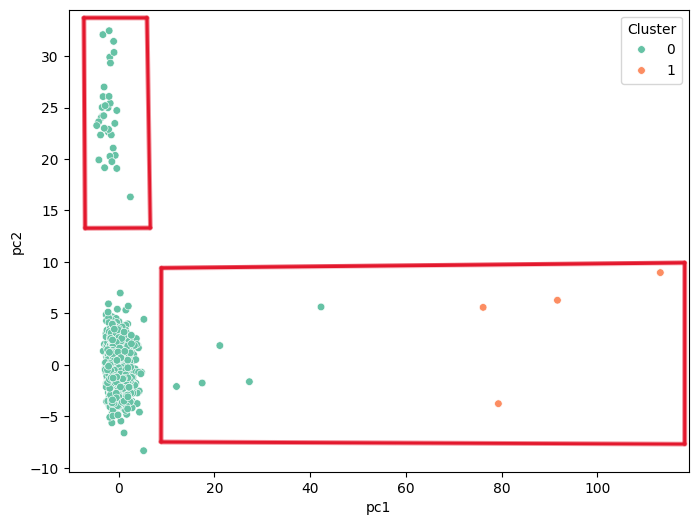
\includegraphics[width=\linewidth]{PCA0r3.png}
\end{minipage}
\hspace{0.3em}
\begin{minipage}{0.55\linewidth}
	\centering
	
\includegraphics[width=\linewidth]{PCA3.png}
\end{minipage}
\end{center}

\small{$$
\begin{array}{c|cccc}
\text{cluster} & 0 & 1 & 2 & 3\\
\hline
y=0 & 513 &  231 & 523 & 163\\
y=1 & 39 & 12 & 32 & 12 \\
\end{array}
$$}

\end{frame}

\begin{frame}{\textbf{Results III}　{0.5test, ns=3, 5-folds cv - mean}}
\linespread{0.9}

{\small
$$
\begin{array}{l|ccc|ccc}
\text{model} 
& \text{$C_0$ACC} & \text{$C_0$FAR} & \text{$C_0$ROCAU} 
& \text{$C_1$ACC} & \text{$C_1$FAR} & \text{$C_1$ROCAU}\\
\hline
\text{LR}  & 0.8424 & 0.1054 & 0.5277 & 0.9054 & 0.0520 & 0.5073\\
\text{SVM} & 0.9294 & 0.0000 & 0.5000 & 0.9507 & 0.0000 & 0.5000\\
\text{DT}  & 0.8081 & 0.1424 & 0.5038 & 0.9054 & 0.0607 & 0.6030\\
\text{RF}  & 0.9294 & 0.0000 & 0.5000 & 0.9507 & 0.0000 & 0.5000\\
\text{XGB} & 0.9149 & 0.0156 & 0.4922 & 0.9507 & 0.0000 & 0.5000\\
\end{array}
$$
}

{\small
$$
\begin{array}{l|ccc|ccc}
\text{model} 
& \text{$C_2$ACC} & \text{$C_2$FAR} & \text{$C_2$ROCAU} 
& \text{$C_3$ACC} & \text{$C_3$FAR} & \text{$C_3$ROCAU}\\
\hline
\text{LR}  & 0.8955 & 0.0650 & 0.5937 & 0.8743 & 0.0862 & 0.6236\\
\text{SVM} & 0.9423 & 0.0000 & 0.5000 & 0.9314 & 0.0000 & 0.5000\\
\text{DT}  & 0.8595 & 0.0956 & 0.5094 & 0.8171 & 0.1225 & 0.4387\\
\text{RF}  & 0.9423 & 0.0000 & 0.5000 & 0.9314 & 0.0000 & 0.5000\\
\text{XGB} & 0.9441 & 0.0019 & 0.5276 & 0.9257 & 0.0062 & 0.4969\\
\end{array}
$$
}

\end{frame}

% --- 結束 ---
\section*{結束}

\begin{frame}[plain] % 產生無外框的頁面
	\begin{center}
		{\Huge The End}
		\bigskip\bigskip 

		{\LARGE Questions  \&  Comments}
	\end{center}
\end{frame}
\end{document}ㄒ
